\documentclass[a4paper, 11pt]{article}
\usepackage{graphicx}
\usepackage{amsmath}
\usepackage[pdftex]{hyperref}
\usepackage{epstopdf}
\usepackage{multirow}
\usepackage[table,xcdraw]{xcolor}

% Lengths and indenting
\setlength{\textwidth}{16.5cm}
\setlength{\marginparwidth}{1.5cm}
\setlength{\parindent}{0cm}
\setlength{\parskip}{0.15cm}
\setlength{\textheight}{22cm}
\setlength{\oddsidemargin}{0cm}
\setlength{\evensidemargin}{\oddsidemargin}
\setlength{\topmargin}{0cm}
\setlength{\headheight}{0cm}
\setlength{\headsep}{0cm}

\renewcommand{\familydefault}{\sfdefault}

\title{Data Mining: Learning from Large Data Sets - Fall Semester 2015}
\author{caifa.zhou@geod.baug.ethz.ch\\ pungast@student.ethz.ch\\ llara@student.ethz.ch\\}
\date{\today}

\begin{document}
\maketitle

\section*{Approximate near-duplicate search using Locality Sensitive Hashing} 

To detect duplicate videos a locality sensitive hashing solution using MapReduce was implemented.
Below, our solution is described in steps.

The \textbf{mapper} reads each line of input, extracts the video ID and shingles, deletes recurring elements in the shingles and sorts the shingles. It then calculates the signature matrix column for each video, partitions it into bands, hashes each band and emits the result.

To calculate the signature matrix columns, we create n hash functions of the form $h_{a,b}(x) = ax + b \bmod N$ (where $N=20001$) by generating parameter vectors $a$ and $b$ of size n containing random nonnegative integers. Using the MinHash approach and each generated $h_{a,b}$, we calculate the column of the signature matrix corresponding to the current video.

To generate candidate pairs, we partition the signature matrix column into $b$ bands and hash each band with a linear hash function (resulting in a bucket ID). The mapper then emits a key-value pair where the key is a string concatentation (band ID + bucket ID) and the value is a tuple (signature matrix column, video ID). In the \textbf{reducer}, all videos that have the same key are then compared pairwise to find out whether the videos were actually similar (with bitwise similarity $\geq 0.9$ in the signature columns of the two videos).

Each machine uses the same seed when generating random numbers for the hash functions.

Given the constraint $ br \leq 1024 $, the parameters $b$ and $r$ were chosen to empirically produce the highest F1-score on the training set, resulting in $(b, r)=(20, 50)$.

The general workflow of the mapper and reducer are illustrated in Figure~\ref{fig: Digraph}. 

\begin{figure}[!htb]
\centering
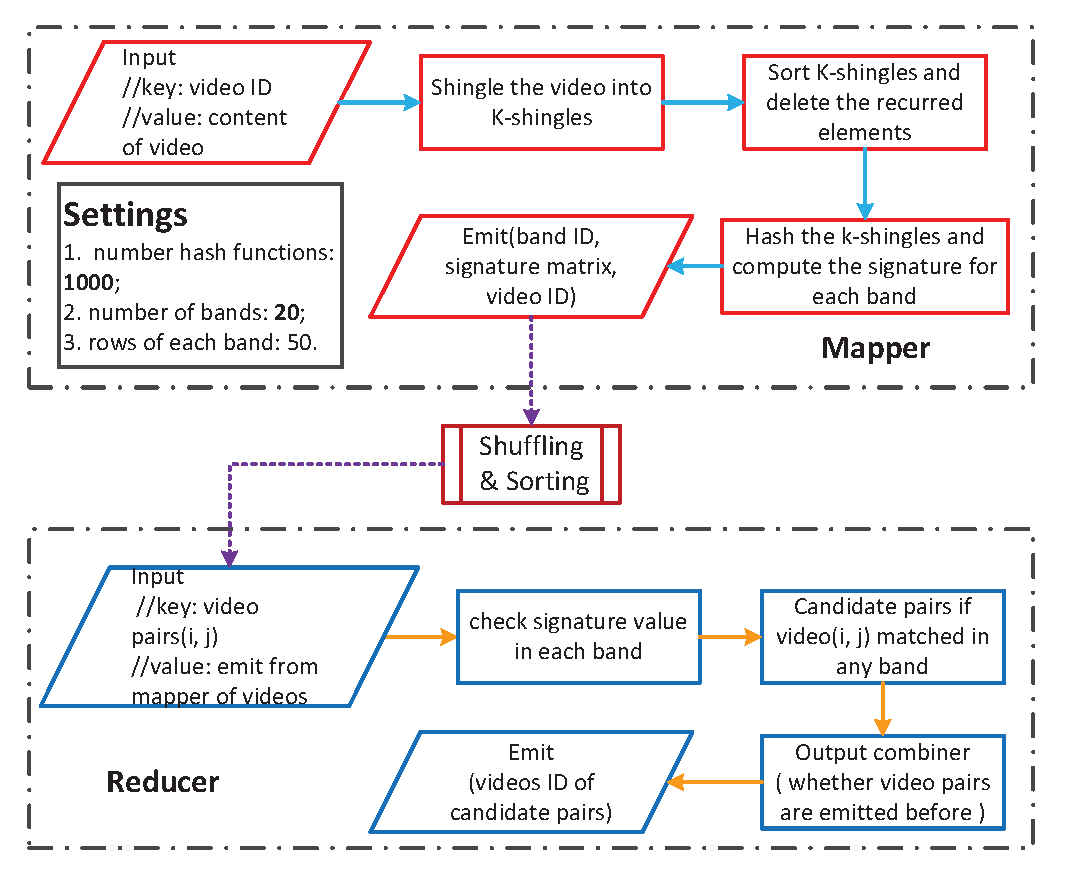
\includegraphics[scale=.7]{workflow_project_1.eps}
\caption{Workflow of the locality sensitive hashing solution using MapReduce.}
\label{fig: Digraph}
\end{figure}

The groupwork was done according to each member's background. First we sat together and discussed the assignment and overall structure, then Caifa Zhou implemented the mapper, Taivo Pungas created the reducer as well as revised the mapper and Lara Lingelbach generated the report. 

\end{document} 
